\section{4 results}
We confirmed that the level of experienced presence impacted spatial exploration behavior in VR. Interestingly the effect was similar across different mazes with a pattern of increasing presence associated with staying in the center of the maze path and spending more time in segments \textit{presumably} critical for navigational success. To emphasize the importance to consider individual differences designing room-scale VR for a broad public, we carved out significant individual characteristics predicting the level of experienced presence, potentially of use directing future design decisions.
\begin{figure}[!t]
\centering
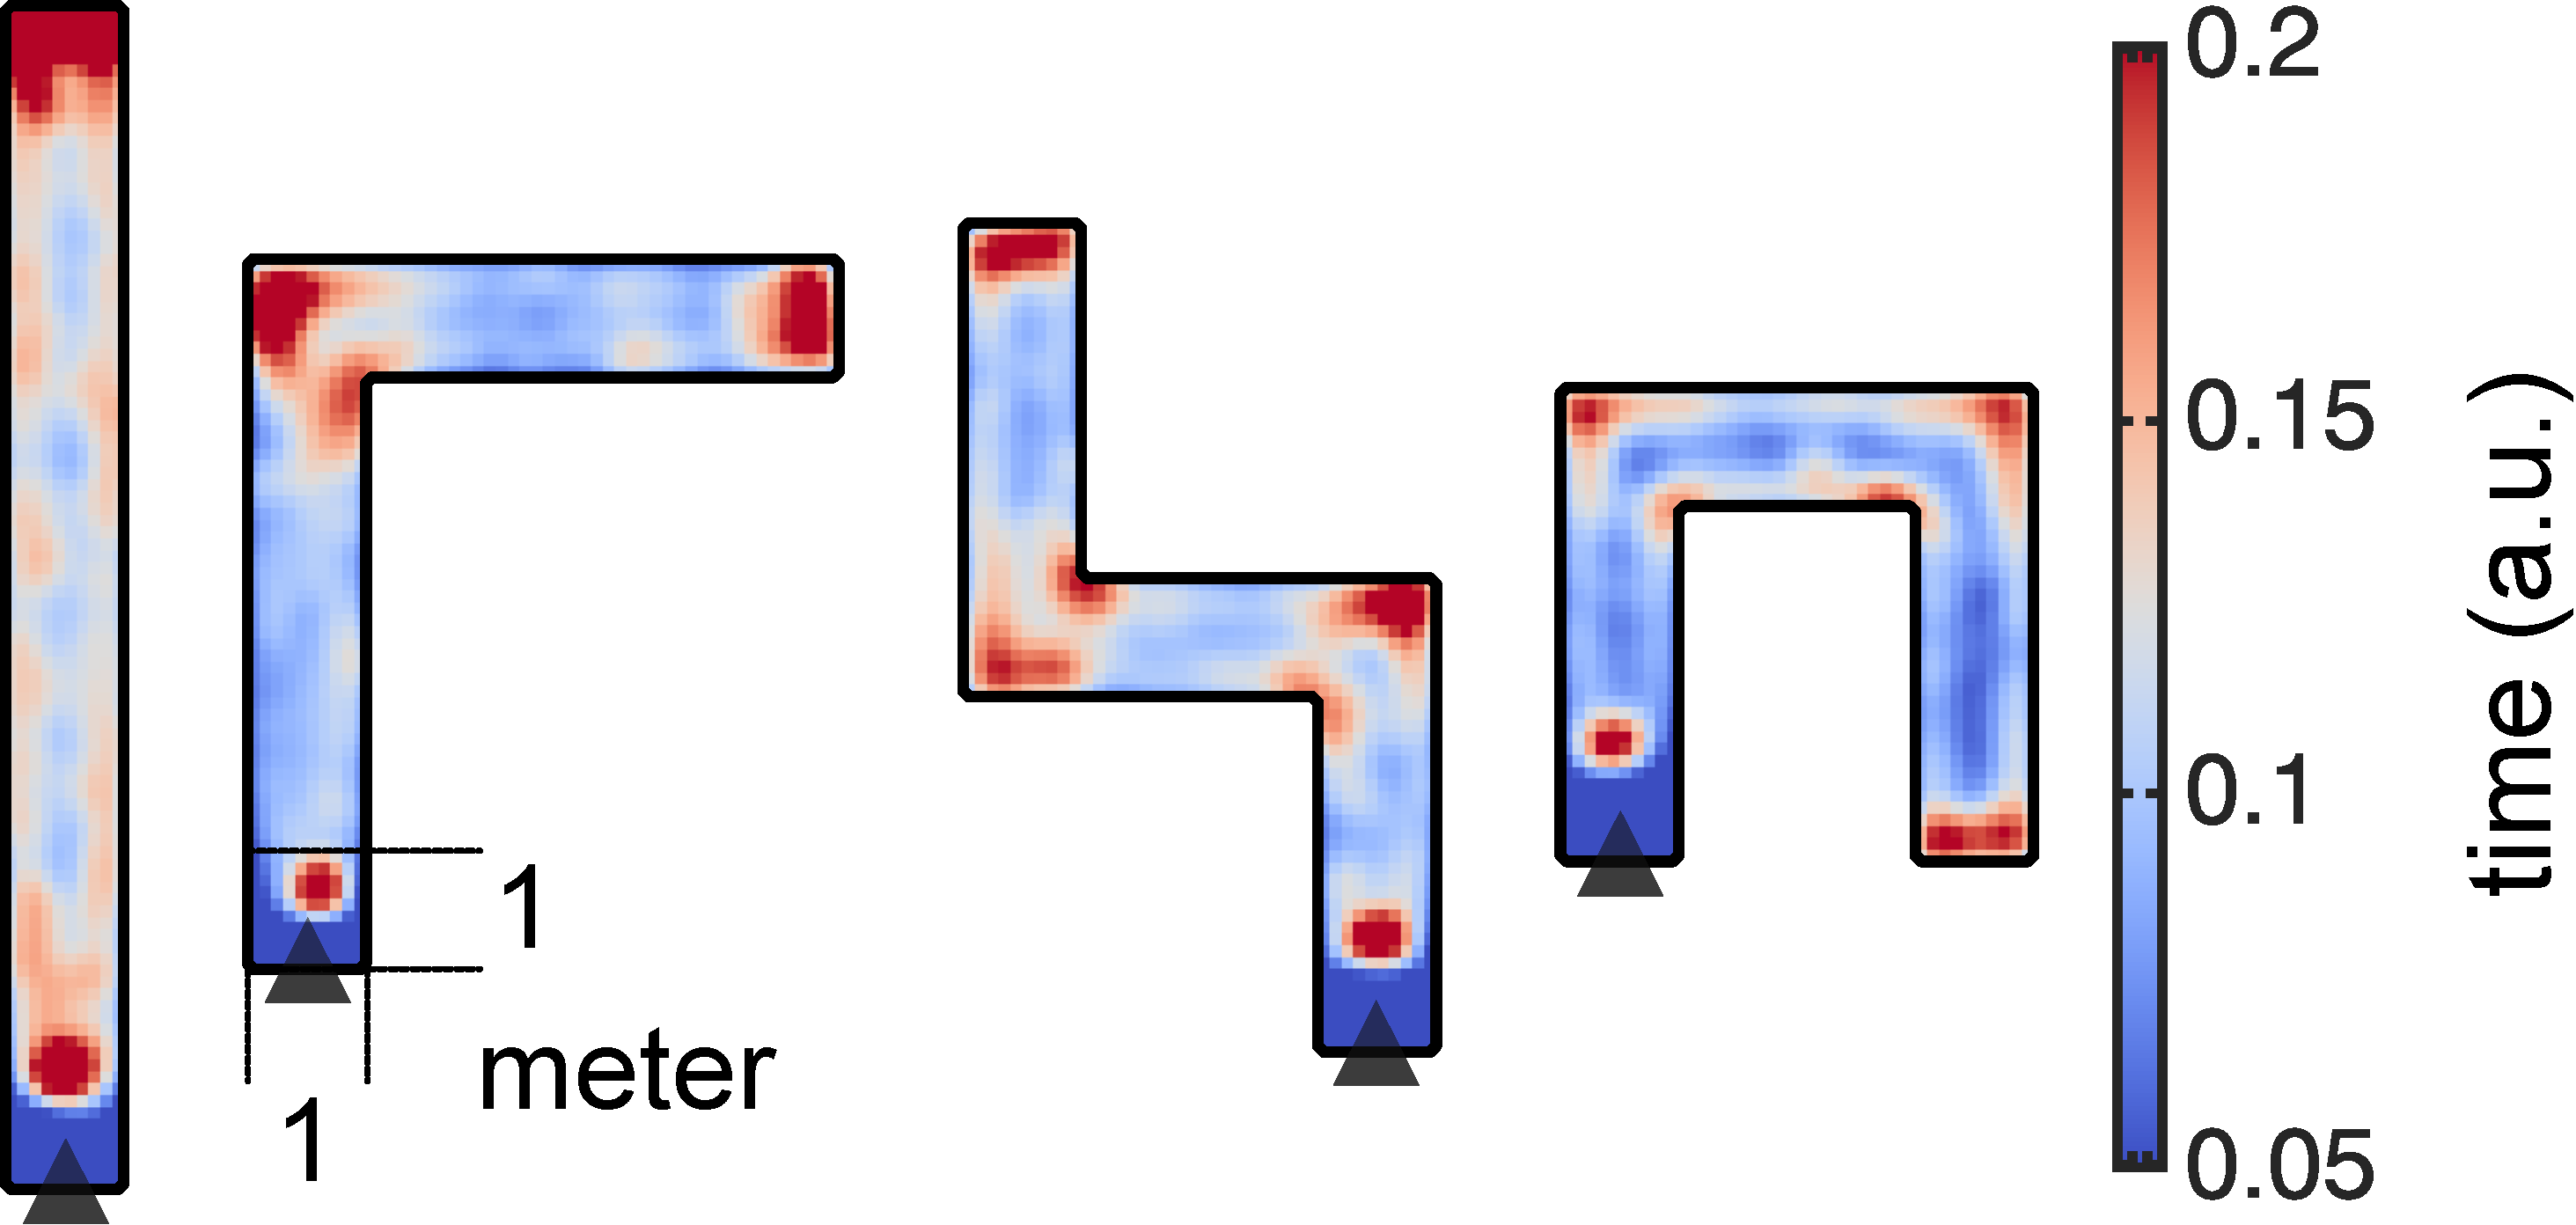
\includegraphics[width=\linewidth]{figures/head_loc_mean.pdf}
\caption{Time spent at each location (grand-average) in each of the four mazes: I, L, Z and U. The whole lab space is roughly 12 by 8 meters in size. Hotter colors, i.e. red, indicate a longer time spent at that location.}
\label{head_loc_mean}
\end{figure}